% 113-01(인쇄 113쪽) — 유형 066 01번의 두 정규분포곡선 A, B(대칭축은 같고 A 가 높고 좁으며 B 가 낮고 넓다 · 대칭축은 점선).
% 스캔 화질이 낮아 TikZ 로 다시 그림. 라벨은 원문에 있는 것만(A, B, x)이고 평균·표준편차의 값은 적지 않는다.
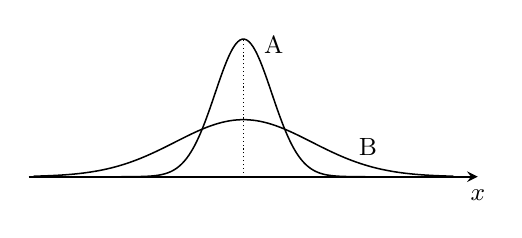
\begin{tikzpicture}[x=0.62cm, y=1.15cm, line width=0.55pt, font=\small]
  \draw[->, >=stealth, line width=0.7pt] (-4.4,0) -- (4.8,0) node[below=1pt] {$x$};
  \draw plot[domain=-2.5:2.5, samples=110, smooth] ({\x},{1.52*exp(-\x*\x/(2*0.58*0.58))});
  \draw plot[domain=-4.3:4.3, samples=110, smooth] ({\x},{0.63*exp(-\x*\x/(2*1.40*1.40))});
  \draw[densely dotted, line width=0.4pt] (0,0) -- (0,1.52);
  \node at (0.62,1.45) {$\mathrm{A}$};
  \node at (2.55,0.33) {$\mathrm{B}$};
\end{tikzpicture}
